\documentclass[twocolumn, a4paper]{icethesisabst}
\usepackage[dvipdfmx]{graphicx}
\usepackage[hang,small,bf]{caption}
\usepackage[subrefformat=parens]{subcaption}
\usepackage{here}
%\renewcommand{\figurename}{Fig.}

\title{{\bf クラスタサイズ調整変数を導入した \\ クラスタリング手法の特性比較及び精度評価}
  {\normalsize \\ Characteristic Comparison and Accuracy Evaluation of Clustering Method \\ with Cluster Size Adjustment Variable}}
  \author{
    AF16009 池辺~颯一 \\ Soichi Ikebe \and
    指導教員 神澤~雄智 \\ Yuchi Kanzawa
  }

\begin{document}
\maketitle


\section{はじめに}
近年,情報通信社会の発展に伴いデータ量が増大し,
日々多様なデータがコンピュータに蓄積されている.
この大量のデータから有益な情報を抽出する手法として,
データを類似度に基づきグループ化するクラスタリングに注目が集まっている.
既存の手法における課題として,各クラスタのサイズに差がある場合,
クラスタリングから有意な結果が得られないというものがある.
そこで,各クラスタのサイズを考慮してクラスタリングを行う手法が複数提案されており,
本研究はそれらの手法について各手法の特性を把握するとともに,
最も有効な手法を発見することを目的とする.


\section{実験内容}
各クラスタのサイズを考慮するために,
既存の手法にクラスタサイズ調整変数を導入した
sFCMA~\cite{sFCMA}, eFCMA~\cite{eFCMA}, qFCMA~\cite{qFCMA}
の3手法について実験を行う.

まず,これらの手法についてそれぞれの特性を把握するため,人工データを用いて実験を行う.
複数のパラメータで実験を行い,それぞれで算出された分類関数~\cite{cFunc}から比較及び評価を行う.
分類関数は,各クラスタに対する帰属度を座標空間上に可視化したもので,分類関数により,
データがどのクラスタに属するかということを調べることができ,新たに与えられたデータ点についても,その帰属度を計算することができる.
分類関数値が,1もしくは0の値に近ければクリスプ,クラスタ数の逆数に近ければファジィという.
したがって,究極的にクリスプな状態ではその分類関数値は1もしくは0の値しか取らず,
究極的にファジィな状態ではその分類関数はクラスタ数の逆数しか取らない.

次に,これらの手法から最も有用なものを発見するために,
実データを用いてAdjusted Rand Index(ARI)~\cite{ARI}を算出する.
ARIは,分類結果の精度評価を$-1$から$1$までの範囲で行う指標で,$1$の時に完全一致,$0$の時にランダムであることを表す.
本研究ではARIの値が最も高いものを有効な手法と評価する.


\section{人工データの実験結果}
人工データとして,
クラス数2,各クラスのデータ数50,合計データ数100のデータを用いた.
各クラスタのデータは,
第$1$クラスタを平均値($-1$, $-1$),標準偏差($0.5$, $0.5$)
第$2$クラスタを平均値($1$, $1$),標準偏差($0.5$, $0.5$)
のガウスサンプリングで生成した.
また,初期値として,帰属度に正解帰属度を与え,クラスタサイズ調整変数にクラスタ数の逆数を与えた.
実験結果の図における垂直軸は帰属度を,底面はデータ空間を表す.
網掛けで示されるのが分類関数であり,各点がデータを表している.
また,分類関数とデータ点は$2$色に別れており,各色が人工データの第$1$クラスタと第$2$クラスタに属することを表している.
分類関数については緑色が第$1$クラスタ,青色が第$2$クラスタに属することを表しており,
データ点については紫色が第$1$クラスタ,黄色が第$2$クラスタに属することを表している.

sFCMAの実験結果を図~\ref{fig:sFCMA-Em2},~\ref{fig:sFCMA-Em11}に示す.
パラメータ$m$を$2.00$から$1.01$に変化させたところ,
分類関数は$m$の値が大きいほどファジィになり,小さいほどクリスプになることが分かった.
次に,eFCMAの実験結果を図~\ref{fig:eFCMA-Lambda1},~\ref{fig:eFCMA-Lambda10}に示す.
パラメータ$\lambda$を$1$から$10$に変化させたところ,
分類関数は$\lambda$の値が小さいほどファジィになり,大きいほどクリスプになることが分かった.
qFCMAの実験結果を図~\ref{fig:qFCMA-Em2-Lambda1},~\ref{fig:qFCMA-Em11-Lambda1},~\ref{fig:qFCMA-Em11-Lambda10}に示す.
こちらは,パラメータ($m$, $\lambda$)の組み合わせとして,$(2.00, 1)$, $(1.01, 1)$, $(1.01, 10)$
の3通りでクラスタリングを行った.
図~\ref{fig:qFCMA-Em2-Lambda1}及び図~\ref{fig:qFCMA-Em11-Lambda1}の分類関数より,
$m$の値が大きいほどファジィになり,小さいほどクリスプになることが分かった.
また,図~\ref{fig:qFCMA-Em11-Lambda1}及び図~\ref{fig:qFCMA-Em11-Lambda10}の分類関数より,
$\lambda$の値が小さいほどファジィになり,大きいほどクリスプになることが分かった.
そして,図~\ref{fig:sFCMA}及び図~\ref{fig:qFCMA-Em2-Lambda1},~\ref{fig:qFCMA-Em11-Lambda1}の分類関数より,
qFCMAにおいて$m-1\rightarrow+0$とするとsFCMAと同じ特性が得られ,
図~\ref{fig:eFCMA}及び図~\ref{fig:qFCMA-Em11-Lambda1},~\ref{fig:qFCMA-Em11-Lambda10}より,
$\lambda\rightarrow\infty$とするとeFCMAと同様の特性を示すことがわかった.
これらの実験結果よりqFCMAはsFCMAとeFCMAの特性を併せ持つと言える.


\begin{figure}[htbp]
 \centering
 \begin{minipage}{0.4\hsize}
  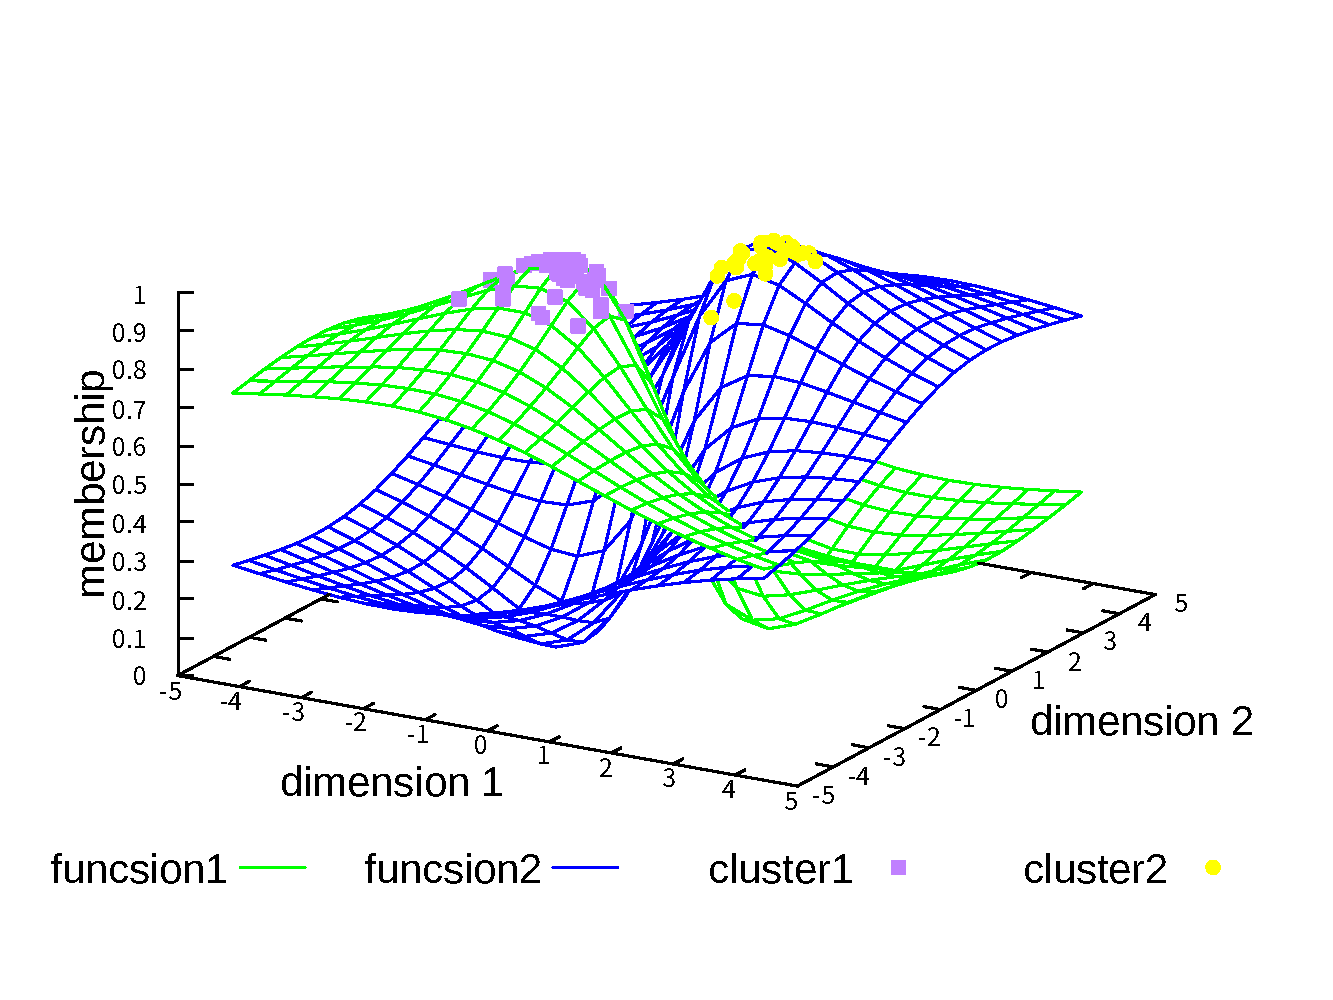
\includegraphics[width=\linewidth]{sFCMA-Em2.pdf}
  \subcaption{$m$=$2.00$}
  \label{fig:sFCMA-Em2}
 \end{minipage}
 \begin{minipage}{0.4\hsize}
  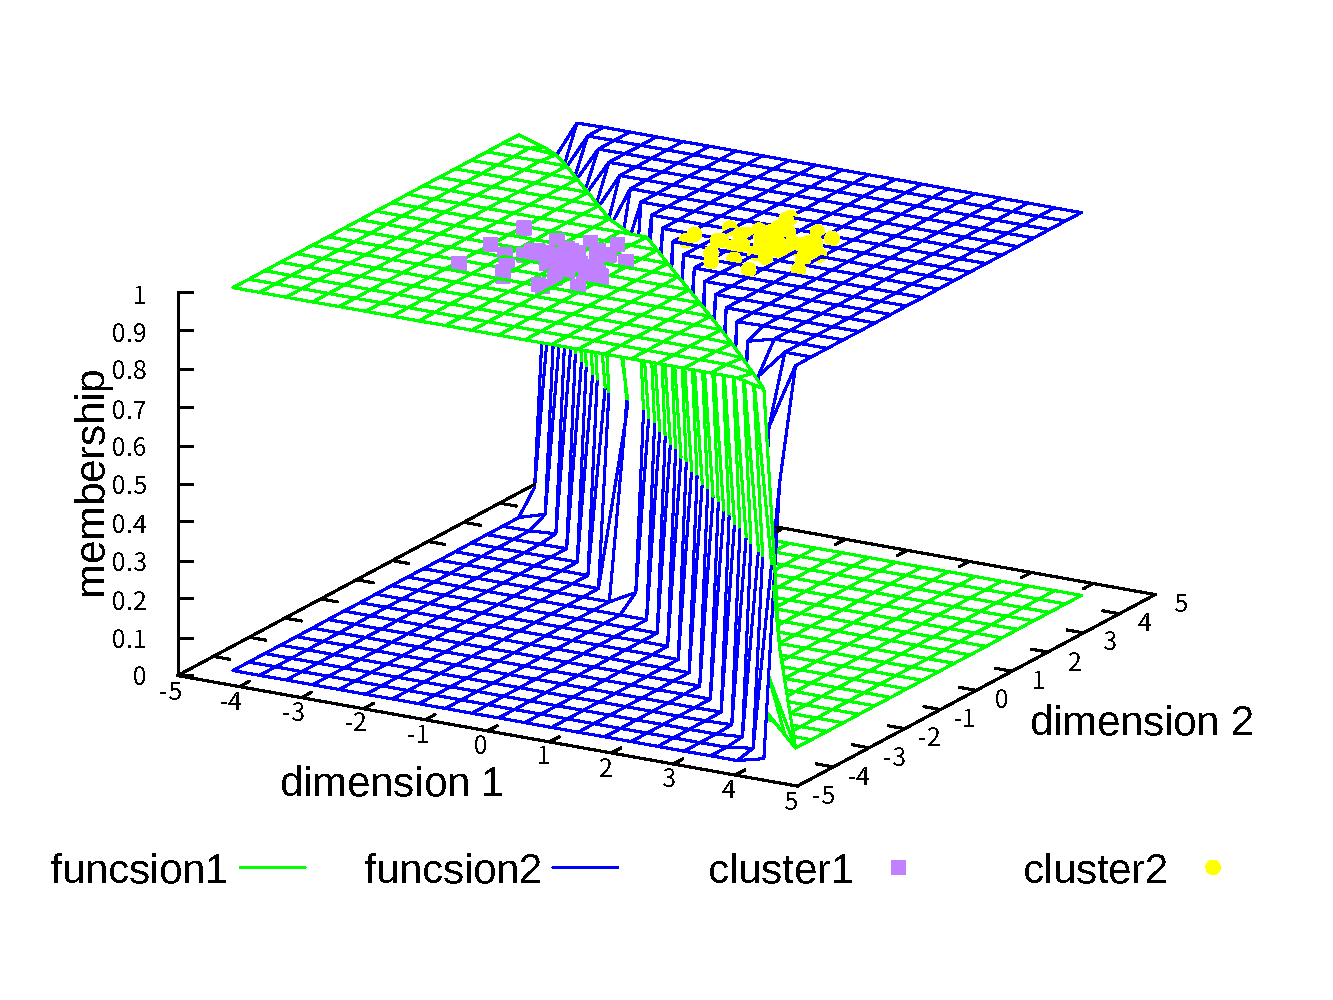
\includegraphics[width=\linewidth]{sFCMA-Em11.pdf}
  \subcaption{$m$=$1.01$}
  \label{fig:sFCMA-Em11}
 \end{minipage}
 \vspace*{0.2cm}
 \caption{sFCMAの人工データの実験結果}
 \label{fig:sFCMA}
\end{figure}

\begin{figure}[htbp]
 \centering
 \begin{minipage}{0.4\hsize}
  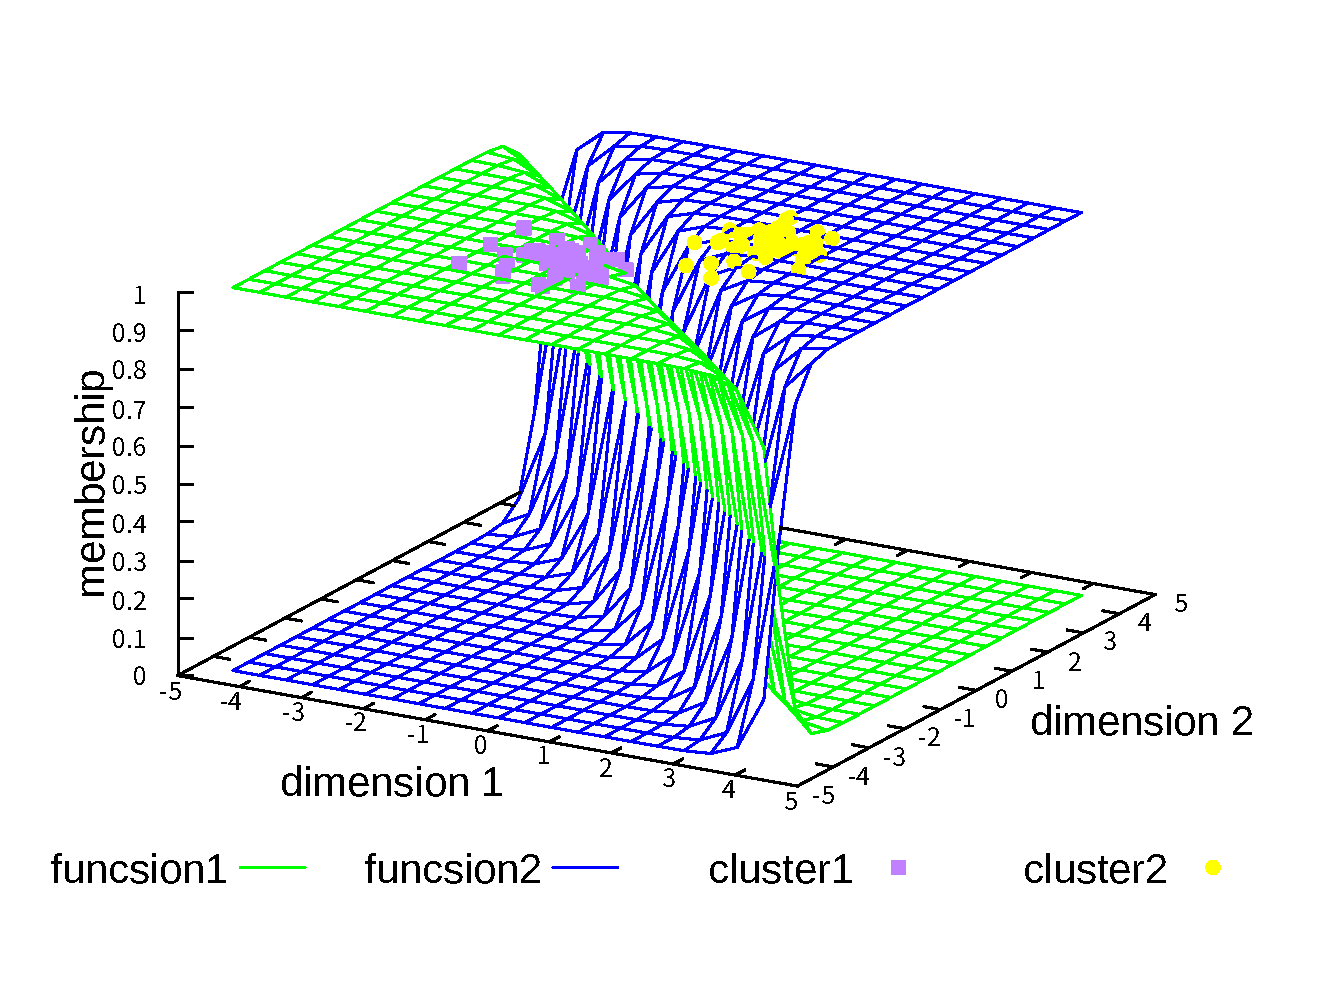
\includegraphics[width=\linewidth]{eFCMA-Lambda1.pdf}
  \subcaption{$\lambda$=$1$}
  \label{fig:eFCMA-Lambda1}
 \end{minipage}
 \begin{minipage}{0.4\hsize}
  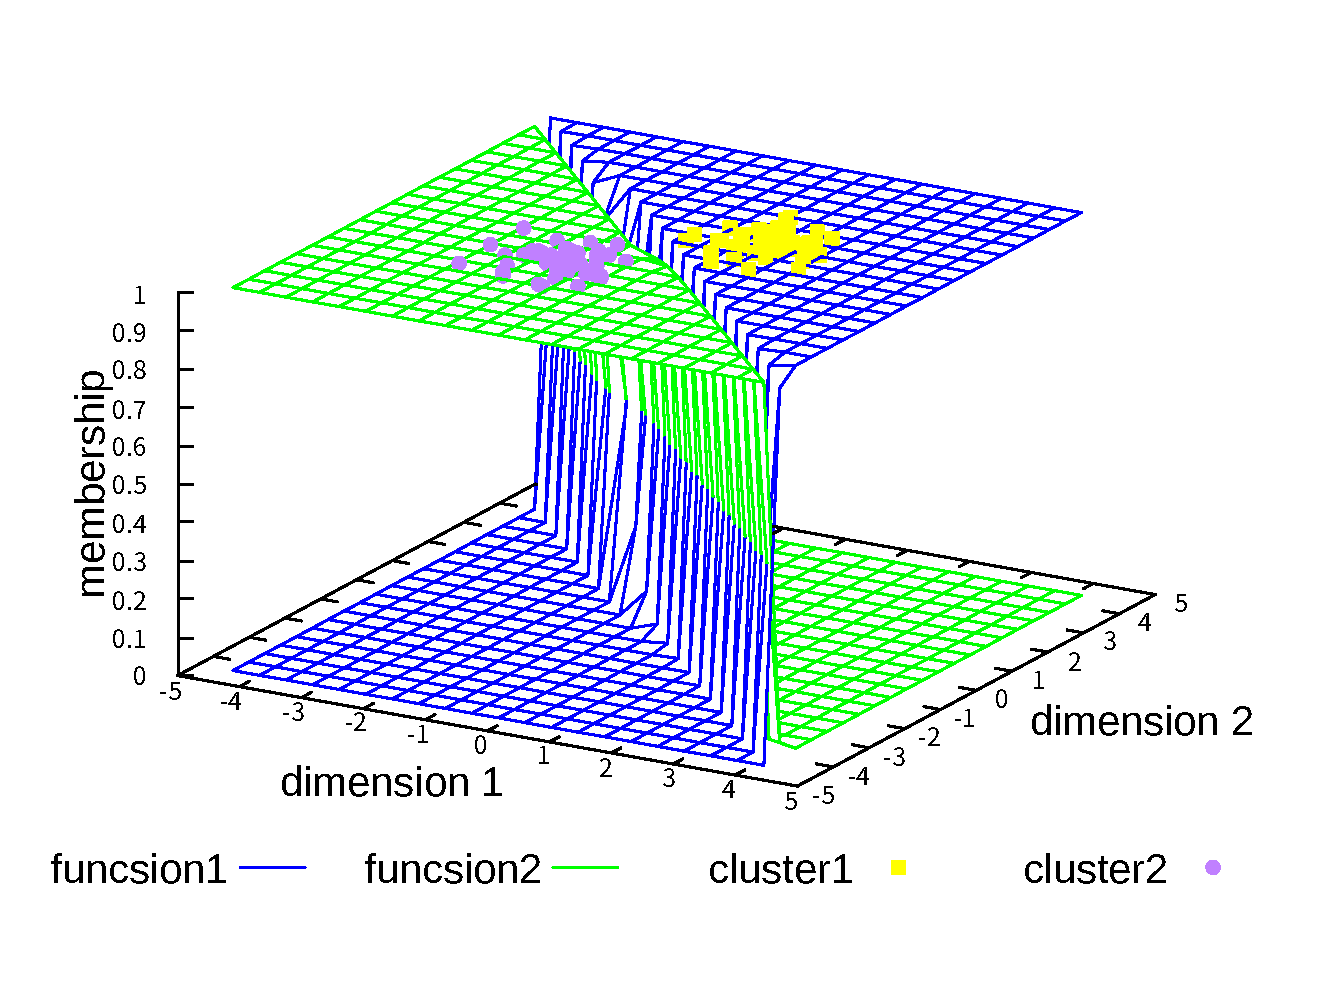
\includegraphics[width=\linewidth]{eFCMA-Lambda10.pdf}
  \subcaption{$\lambda$=$10$}
  \label{fig:eFCMA-Lambda10}
 \end{minipage}
 \vspace*{0.2cm}
 \caption{eFCMAの人工データの実験結果}
 \label{fig:eFCMA}
\end{figure}

\newpage

\begin{figure}[htbp]
 \centering
 \begin{minipage}{0.4\hsize}
  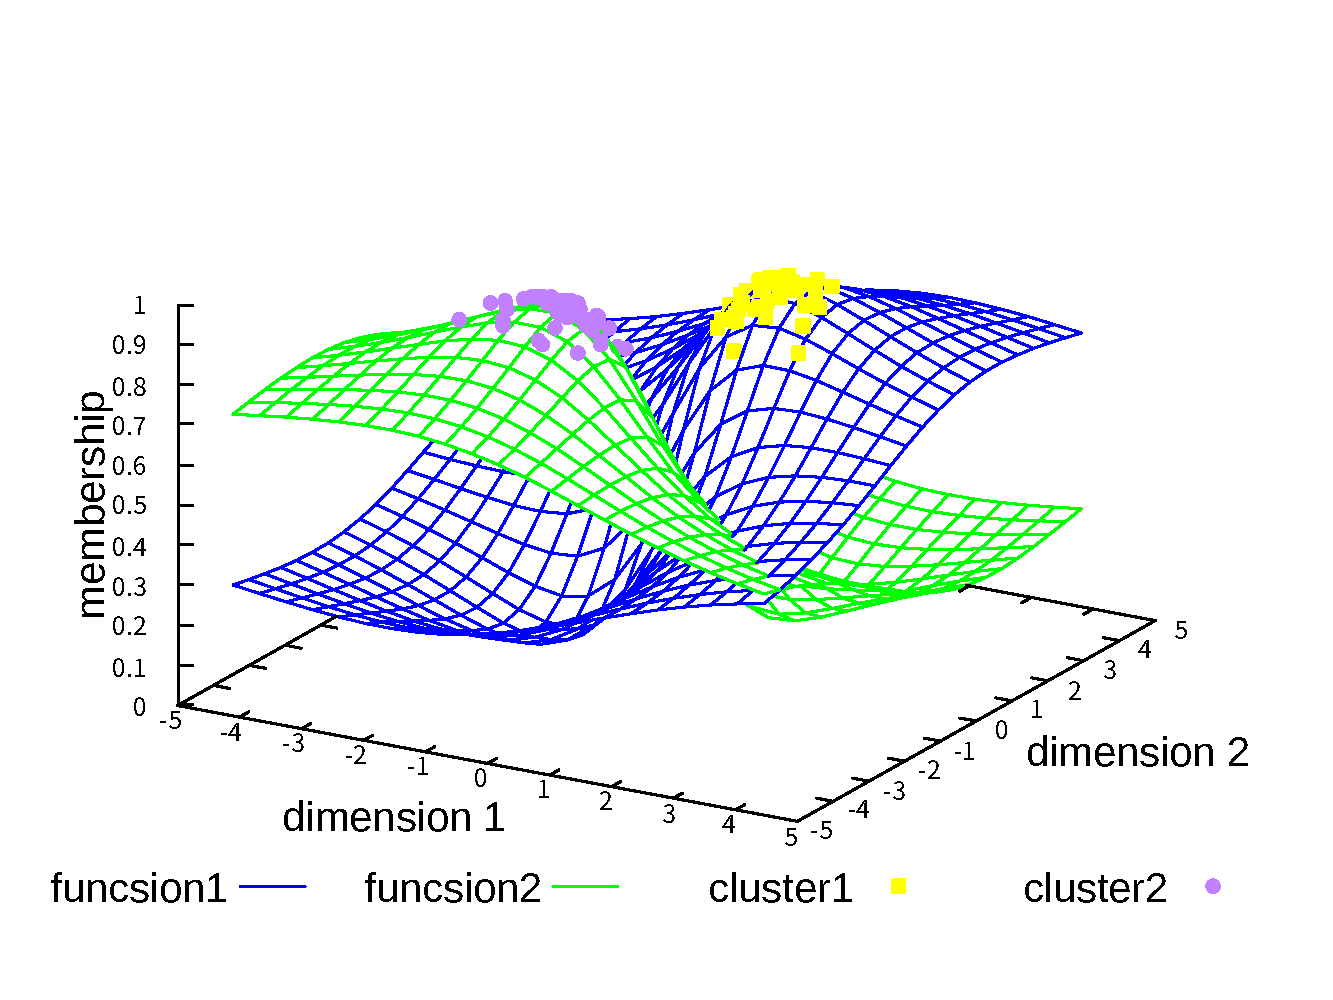
\includegraphics[width=\linewidth]{qFCMA-Em2-Lambda1.pdf}
  \subcaption{$m=2.00, \lambda=1$}
  \label{fig:qFCMA-Em2-Lambda1}
 \end{minipage}
 \begin{minipage}{0.4\hsize}
  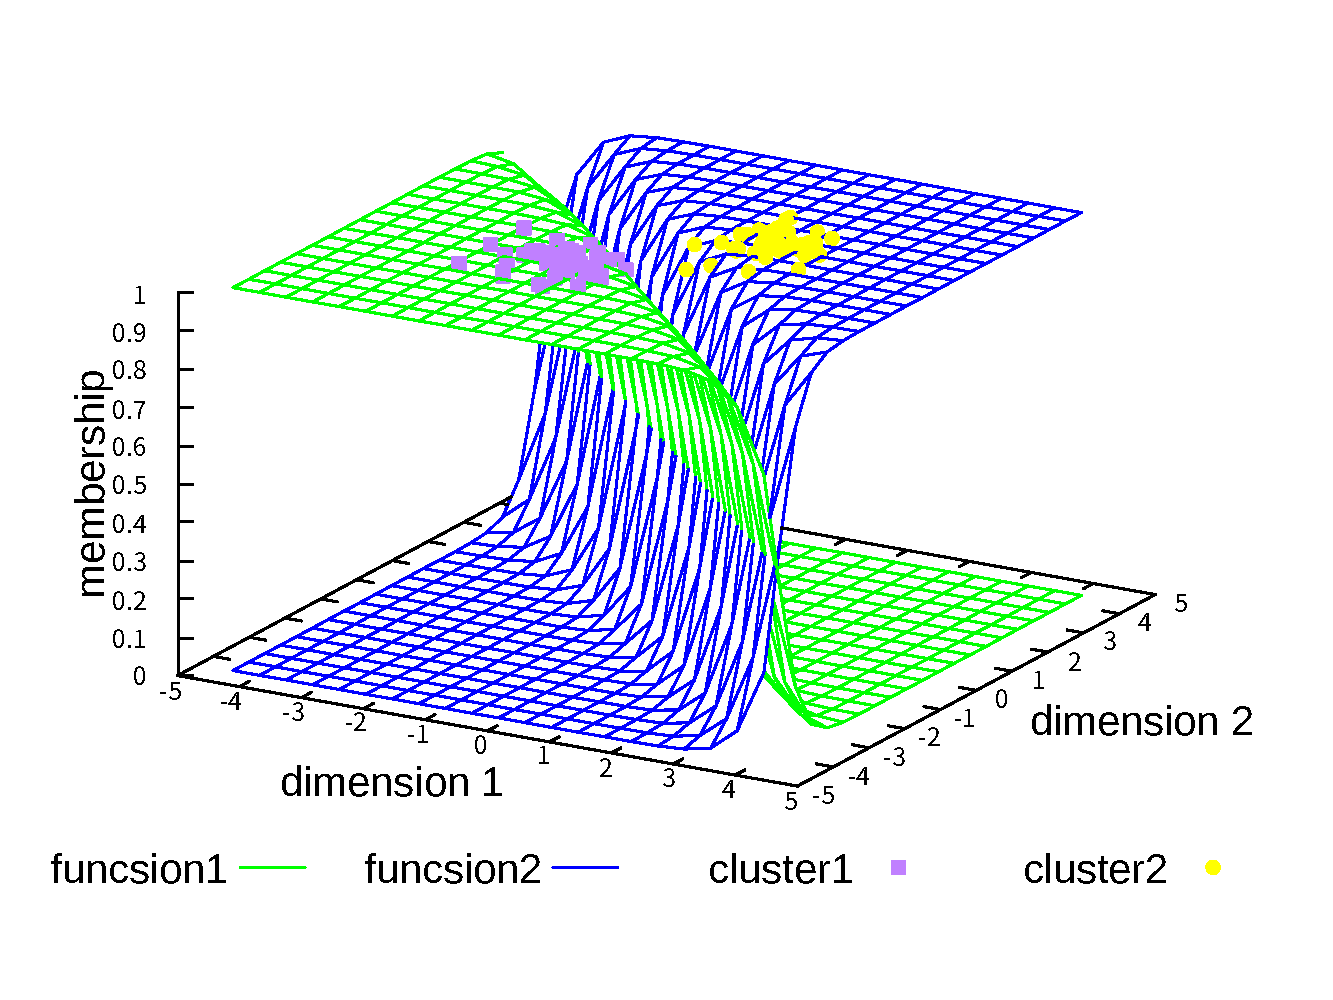
\includegraphics[width=\linewidth]{qFCMA-Em11-Lambda1.pdf}
  \subcaption{$m=1.01, \lambda=1$}
  \label{fig:qFCMA-Em11-Lambda1}
 \end{minipage}
 \begin{minipage}{0.4\hsize}
  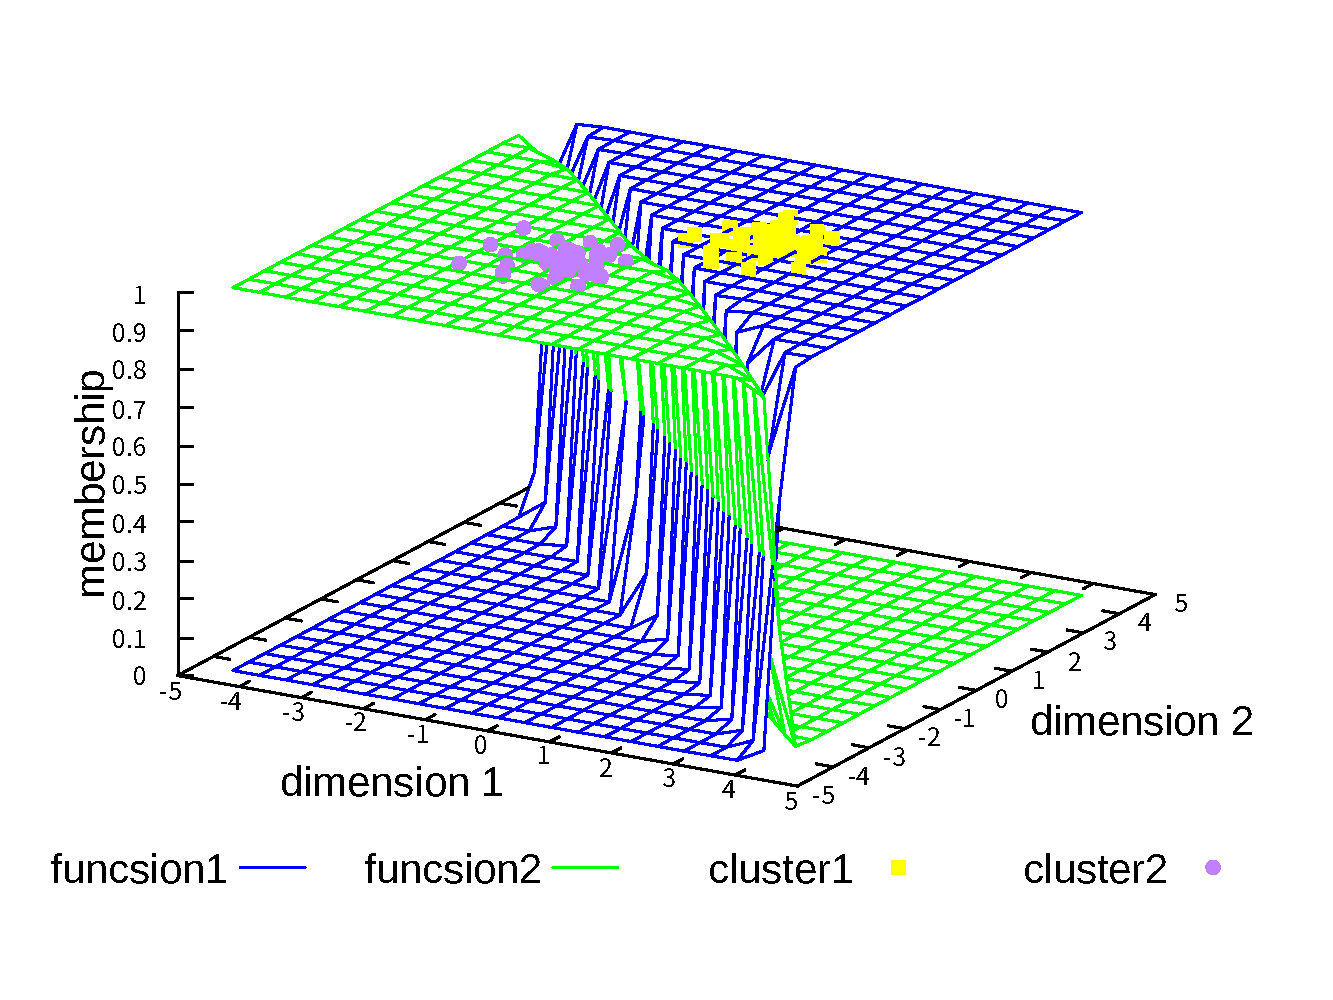
\includegraphics[width=\linewidth]{qFCMA-Em11-Lambda10.pdf}
  \subcaption{$m=1.01, \lambda=10$}
  \label{fig:qFCMA-Em11-Lambda10}
 \end{minipage}
 \vspace*{0.2cm}
 \caption{qFCMAの人工データの実験結果}
 \label{fig:qFCMA}
\end{figure}


\section{実データの実験結果}
実データとしては,
個体数403,
クラス数4の,
被験者の勉強時間や試験結果などの5属性を収録した
``User Knowledge Modeling Dasta Set''
を用いた.
また,初期値として,それぞれのデータの帰属度に正解の帰属度を与え,クラスタサイズ調整変数にクラスタ数の逆数を与えた.
sFCMA, eFCMA, qFCMAの実データ実験の結果について,
それぞれ図~\ref{fig:sFCMA_ARI},~\ref{fig:eFCMA_ARI},~\ref{fig:qFCMA_ARI}に示す.
sFCMAでは$m$の値を$1.1$から$3.0$まで$0.1$刻み,
eFCMAでは$\lambda$の値を$1$から$100$まで$1$刻み,
qFCMAでは$m$の値を$1.1$から$3.0$まで$0.1$刻み,$\lambda$の値を$1$から$100$まで$1$刻みで変化させた.

\begin{figure}[htbp]
 \centering
 \begin{minipage}{0.43\hsize}
  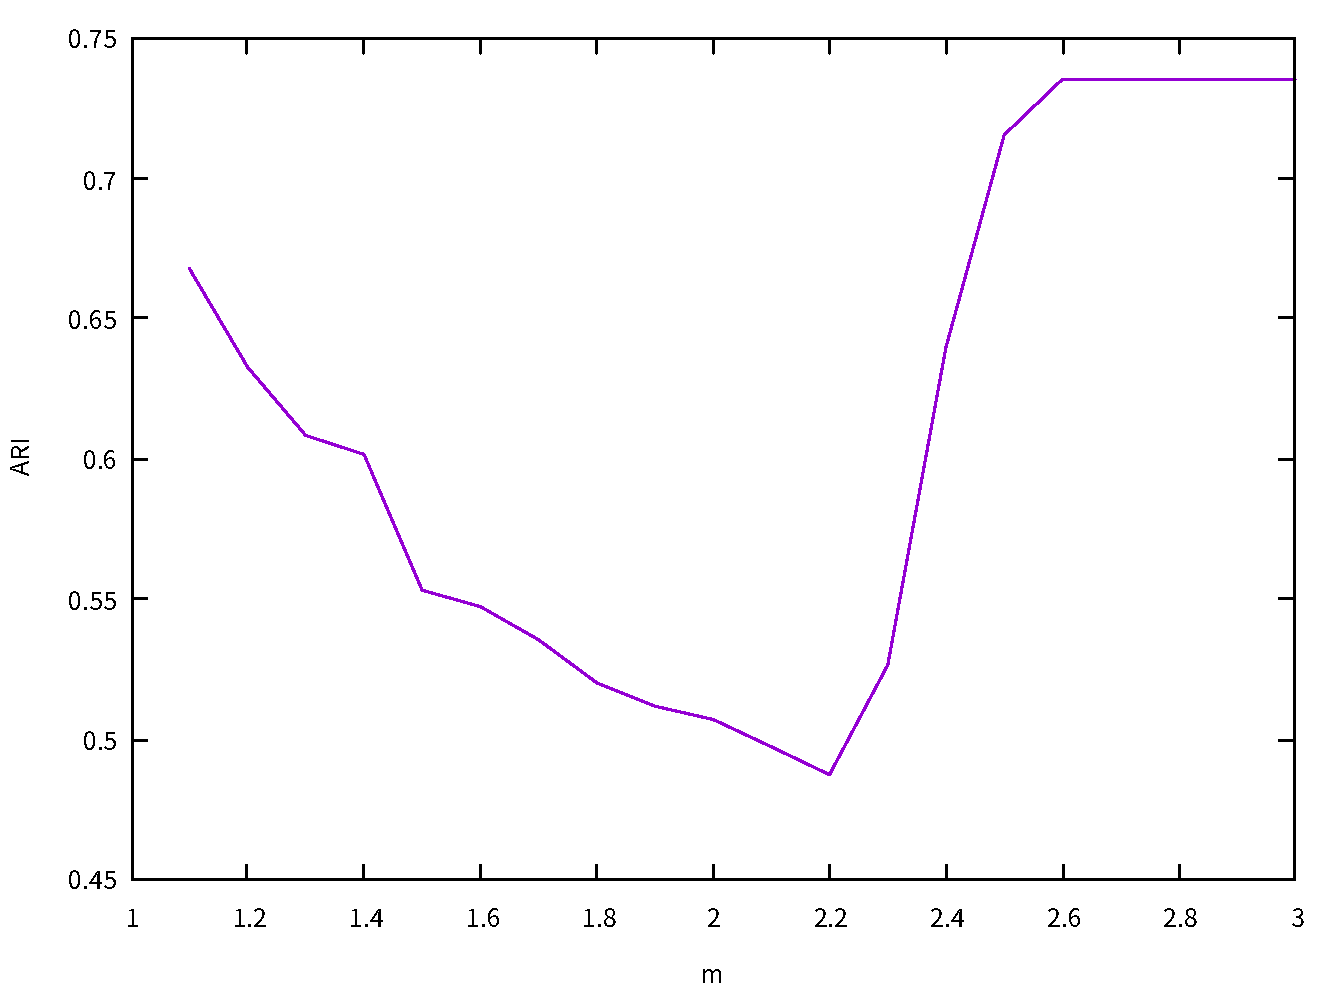
\includegraphics[width=\linewidth]{sFCMA_ARI.pdf}
  \caption{sFCMAの実データの実験結果}
  \label{fig:sFCMA_ARI}
 \end{minipage}
 \begin{minipage}{0.43\hsize}
  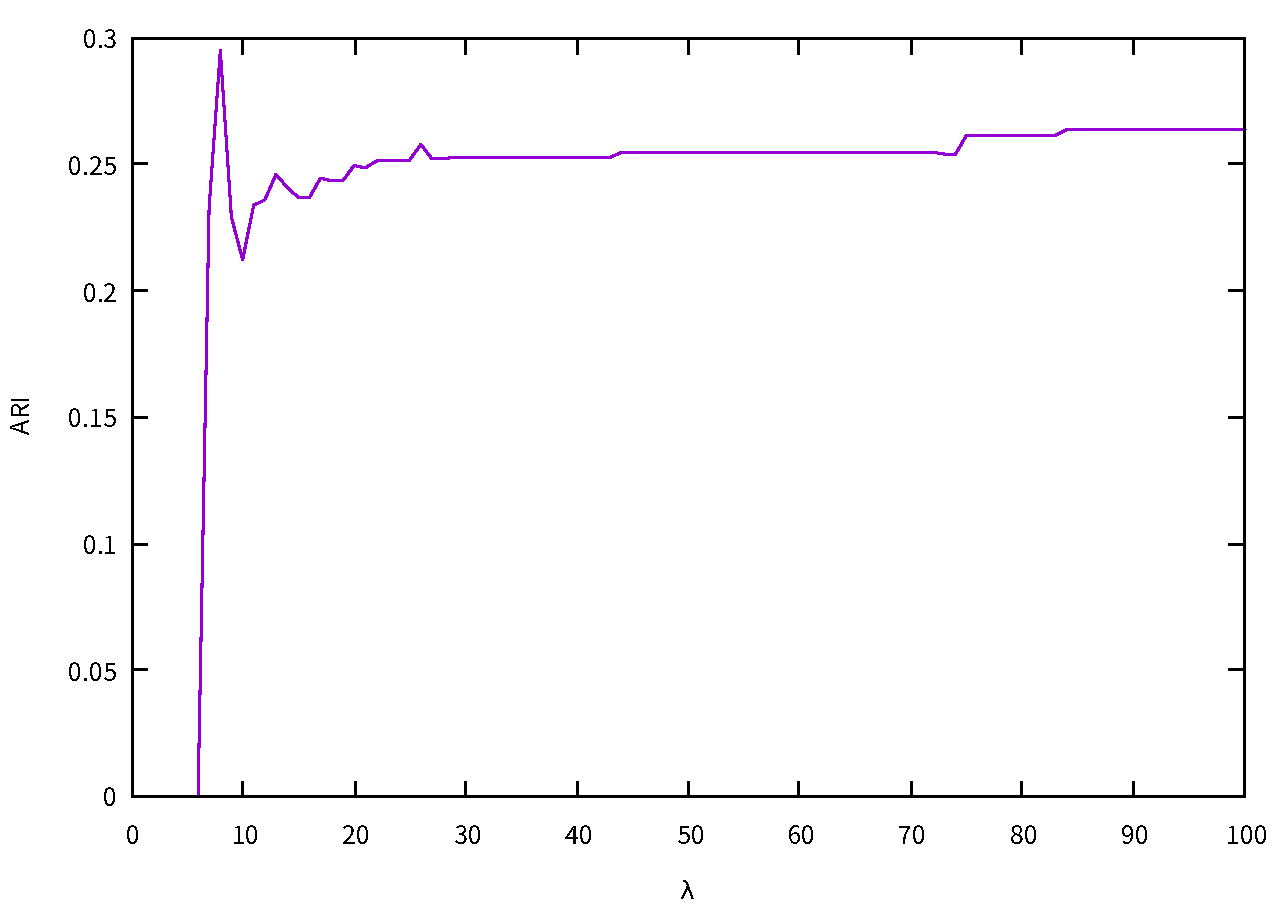
\includegraphics[width=\linewidth]{eFCMA_ARI.pdf}
  \caption{eFCMAの実データの実験結果}
  \label{fig:eFCMA_ARI}
 \end{minipage}
 \begin{minipage}{0.43\hsize}
  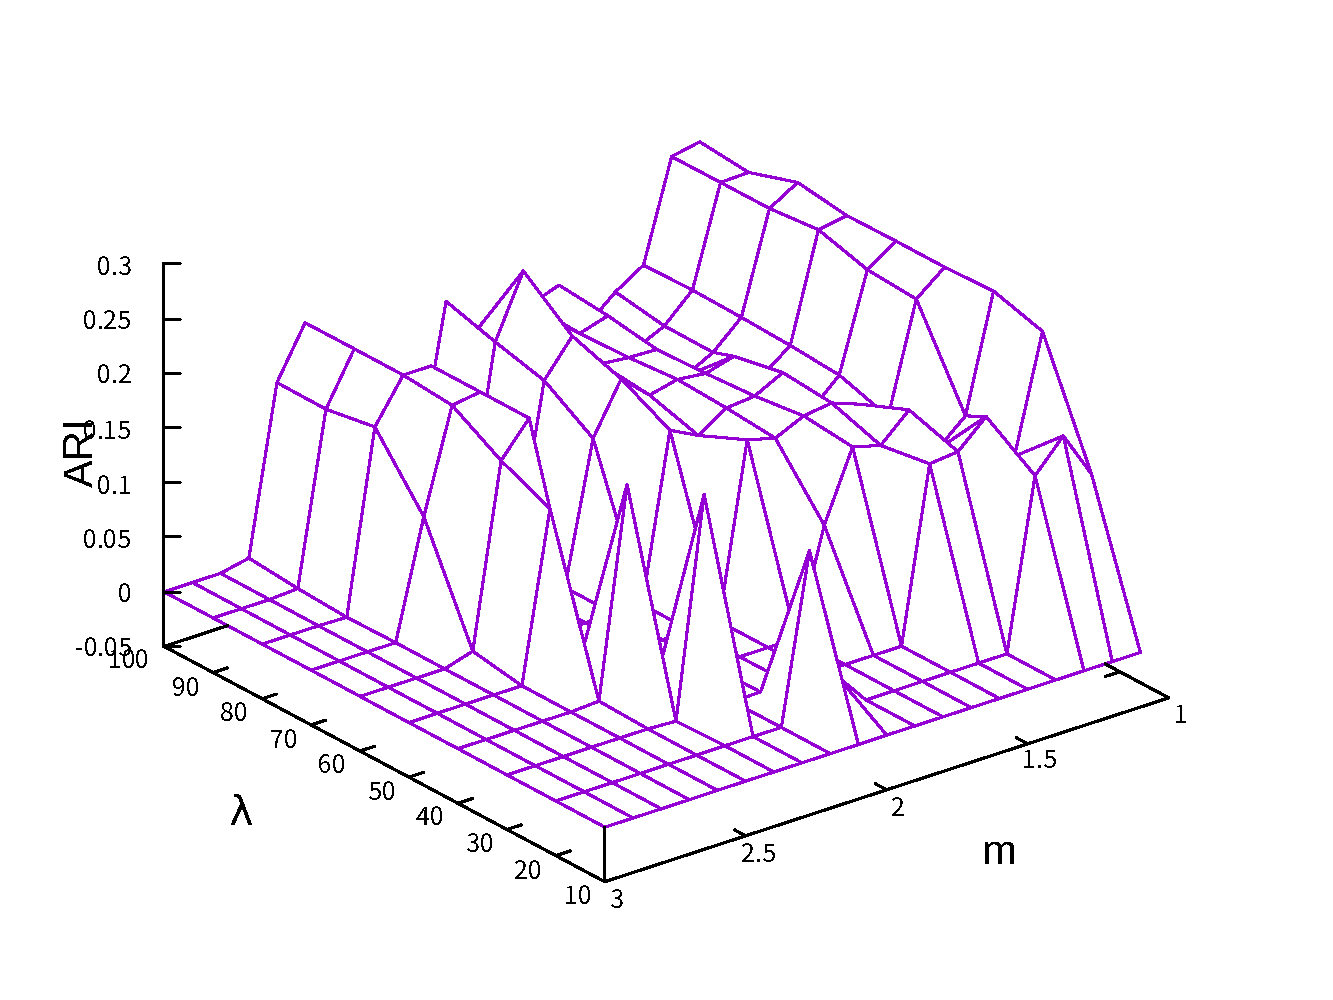
\includegraphics[width=\linewidth]{qFCMA_ARI.pdf}
  \caption{qFCMAの実データの実験結果}
  \label{fig:qFCMA_ARI}
 \end{minipage}
\end{figure}
  
それぞれの手法の最高ARIを表~\ref{tbl:max_ari}に示す.
最も高いARIを示した手法はsFCMAであり,他の$2$手法と比較してARIに$0.4$以上の差が見られた.

\vspace{0.2cm}
\begin{table}[htbp]
 \centering
 \caption{各手法のARIの最高値とパラメータ}
 \begin{center}
  \begin{tabular}{ c || c | c }\hline
   手法名 & ARIの最高値 & パラメータ値\\ \hline \hline
   sFCMA & $0.73515$ & $m = 3$\\ \hline
   eFCMA & $0.29500$& $\lambda = 8$\\ \hline  
   qFCMA & $0.26286$ & $\lambda = 80$, $m = 1.1$\\  \hline
  \end{tabular}
  \label{tbl:max_ari}
 \end{center}
\end{table}


\section{まとめと今後の課題}
既に提案されていた3種のクラスタリング手法の特性と精度について現在に至るまで明らかになっていなかったため,本研究では,人工データを用いた特性比較及び実データを用いた精度比較を行った.
その結果として,
sFCMAは$m$が大きくなるとファジィになり,
eFCMAは$\lambda$が大きくなるほどクリスプになることが分かった.
また,qFCMAはsFCMAとeFCMAの両方の特性を併せ持つということが分かった.
精度はsFCMAが最も高評価となった.要因として,この手法の最適化問題にエントロピー項が含まれないということが考えられる.sFCMAの精度には,エントロピー項が含まれるeFCMA, qFCMAの2手法と比較して大きな差が見られた.
今後の課題は,今回用いなかった他の実データで$3$手法の比較を行い,精度についての裏付けを行うことである.


\begin{thebibliography}{5}
\bibitem{sFCMA}Miyamoto, S., Kurosawa, N.: ``Controlling Cluster Volume Sizes in Fuzzy c-means Clustering'', Proc.~SCIS\&ISIS2004, pp.~1--4, (2004).
\bibitem{eFCMA}Ichihashi, H., Honda, K., Tani, N.: ``Gaussian Mixture PDF Approximation and Fuzzy c-means Clustering with Entropy Regularization'', Proc.~4th Asian Fuzzy System Symposium, pp.~217--221, (2000).
\bibitem{qFCMA}Miyamoto, S., Ichihashi, H., and Honda, K.: Algorithms for Fuzzy Clustering, Springer (2008).
\bibitem{cFunc}宮本 定明, 馬屋原 一孝, 向殿 政男:``ファジイ $c$-平均法とエントロピー正則化法におけるファジィ分類関数'', 日本ファジィ学会誌 Vol.~10, No.~3  pp.~548--557, (1998).
\bibitem{ARI} Hubert, L., and Arabie, P.:``Comparing Partitions'', Journal of Classifcation, Vol.~2, No.~1, pp.~193--218, (1985).
\end{thebibliography}


\end{document}
